\documentclass[12pt,a4paper,UTF8]{article}
\usepackage{ctex}
\usepackage{gbt7714}
\usepackage{amsmath}
\usepackage{mathrsfs}
\usepackage{amssymb}
\usepackage{bm}	
\usepackage{graphicx}% 图片宏包
\usepackage{subfigure}
\usepackage[subfigure]{tocloft}% 在该模板内必须加这句,否则和其他宏包有冲突

\renewcommand{\contentsname}{\vspace*{9.8mm}\zihao{3}\heiti\textbf{目}\hspace{5.8mm}\textbf{录}}

\usepackage{natbib}
\usepackage{setspace}
\setlength{\bibsep}{0em}
\setcounter{secnumdepth}{2}
\setcounter{tocdepth}{2}
%引导点
\renewcommand{\cftdot}{…}
\renewcommand{\cftdotsep}{-0.3}
\renewcommand{\cftsecleader}{\songti\;\cftdotfill{\cftdotsep}}
\renewcommand{\cftsubsecleader}{\songti\;\cftdotfill{\cftdotsep}}
\renewcommand{\cftsubsubsecleader}{\songti\;\cftdotfill{\cftdotsep}}
%缩进
\renewcommand{\cftsubsecindent}{\cftsecindent}
\renewcommand{\cftsubsubsecindent}{\cftsecindent}
%字体
\renewcommand{\cftsecfont}{\zihao{3}\heiti}
\renewcommand{\cftsubsecfont}{\zihao{-3}\heiti}
\renewcommand{\cftsubsubsecfont}{\zihao{4}\heiti}
\renewcommand{\cftsecpagefont}{\zihao{3}\heiti}
\renewcommand{\cftsubsecpagefont}{\zihao{-3}\heiti}
\renewcommand{\cftsubsubsecpagefont}{\zihao{4}\heiti}
%行间距(规范中未对目录不同项之间的间距做规定,以下数值取半倍行高)
\renewcommand{\cftbeforesecskip}{8pt}
\renewcommand{\cftbeforesubsecskip}{7.5pt}
\renewcommand{\cftbeforesubsubsecskip}{7pt}

% %title
\usepackage{titlesec}
\titleformat{\section}{\centering\zihao{3}\bfseries\heiti}{\thesection}{1em}{}
\titleformat{\subsection}{\zihao{-3}\bfseries\heiti}{\thesubsection}{1em}{}
\titleformat{\subsubsection}{\zihao{4}\bfseries\heiti}{\thesubsubsection}{1em}{}

\usepackage{booktabs}
\usepackage{enumerate}

\usepackage{newtxtext}
\usepackage[top=2.5cm, bottom=2.5cm, left=2.5cm, right=2cm]{geometry}

\makeatletter
\@addtoreset{equation}{section}
\makeatother
\renewcommand\theequation{\arabic{section}-\arabic{equation}}

\begin{document}
\setlength{\baselineskip}{20pt}

%%中文摘要

\setcounter{page}{1}

\begin{center}
%一行
\vspace*{1.3mm}
{\heiti\zihao{3}\textbf{论文题目}}\\
\vspace{11mm}

{\zihao{-3}\heiti
\textbf{摘}\hspace{5.3mm}\textbf{要}}
\end{center}
\vspace{4.5mm}
{\zihao{4}
\noindent\phantom{空格}%修改你的中文摘要:
在这里写摘要
}

\vspace{11.5mm}%这一行前后的要留空白行!

\noindent\phantom{空格}{\heiti\textbf{%修改你的关键词
	关键词:}{\songti 关键词,关键词,关键词,关键词
}}


\newpage

\begin{center}
	\vspace*{-3.8mm}
	{\zihao{3}\textbf{Name of Thesis}}\\
	\vspace{20.5mm}
	{\zihao{-3}
	\textbf{ABSTRACT}}
\end{center}
\vspace{7.6mm}
{\zihao{4}
\noindent\phantom{空格}%修改你的摘要
Here is your English Abstrct}

\vspace{16.2mm}
\noindent\hspace{10.6mm}
\textbf{KEY WORDS:} {key word, key word, key word, key word}


\newpage


\setcounter{page}{1}

{\centering\tableofcontents}
\newpage

\setcounter{page}{1}

\section{节标题}
\subsection{节标题}

\newpage

\section{一些例子}
\subsection{文献引用例子}

文献\cite{AlexNet}

文献\cite{VGG,ResNet}

\newpage

\subsection{子图例子}

引用图\ref{fig:subfigure}
引用子图\ref{fig:sub1}

\begin{figure}[htbp]
	\centering
	\subfigure[子图1]
	{
		\label{fig:sub1}		
		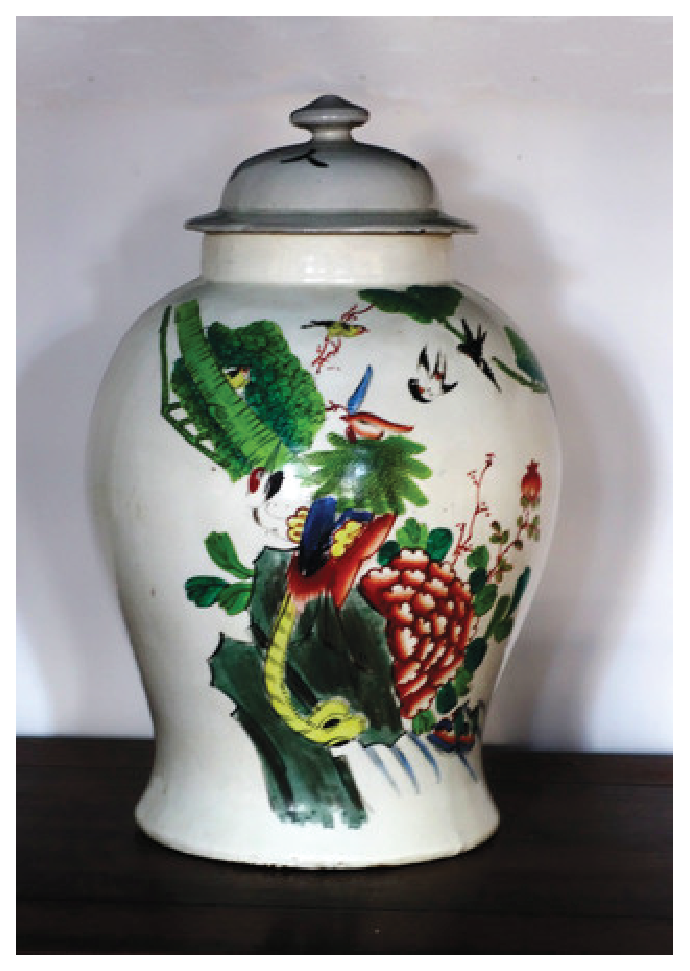
\includegraphics[width=0.45\textwidth]{Figures/figunwave.eps}
	}
	\subfigure[子图2]
	{
		\label{fig:sub2}		
		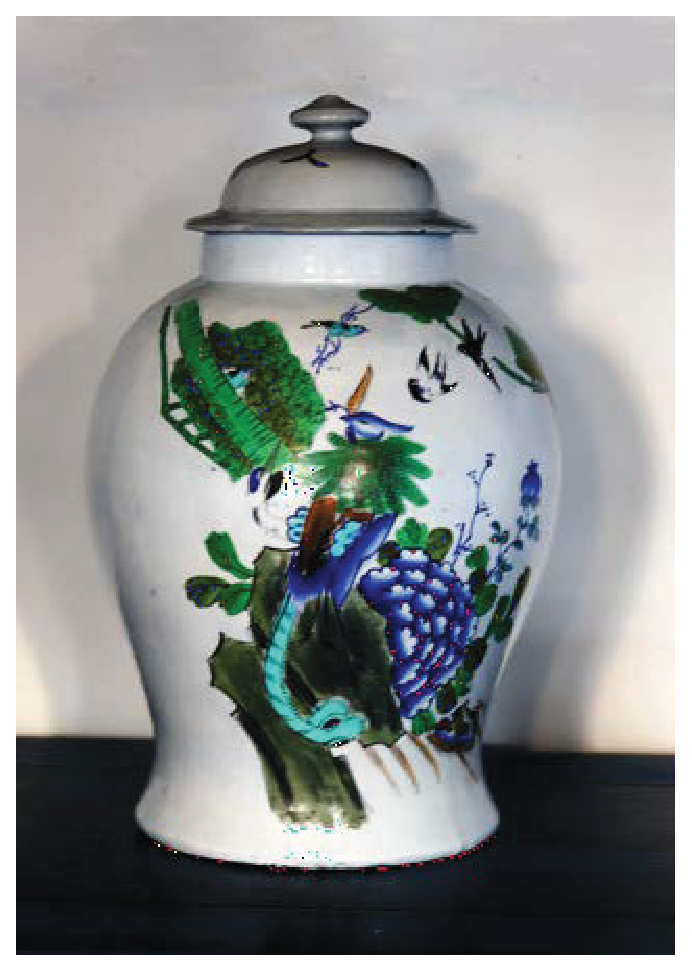
\includegraphics[width=0.45\textwidth]{Figures/figwave.eps}
	}
	\caption{子图示例}
	\label{fig:subfigure}
\end{figure}


\newpage
\addcontentsline{toc}{section}{参考文献}

%\bibliographystyle{unsrt}
\bibliographystyle{gbt7714-numerical}

{\zihao{5}\setlength{\baselineskip}{20pt}
\bibliography{ExampleBib.bib}
}


\newpage
\addcontentsline{toc}{section}{致谢}
\begin{center}
	\vspace*{-2mm}
	\heiti\zihao{3}\textbf{致\hspace{5.7mm}谢}
\end{center}

在这里写致谢

\vspace{5.7cm}\hspace{12.1cm}
{\heiti\zihao{3}\setlength{\baselineskip}{16pt}\selectfont作者名字

\vspace{0.4cm}\hspace{11.4cm}
20XX 年 某 月}

\end{document}